\documentclass[10pt,onecolumn,journal,draftclsnofoot]{IEEEtran}
\usepackage[margin=0.75in]{geometry}
\usepackage{listings}
\usepackage{color}
\usepackage{longtable}
\usepackage{graphicx}
\usepackage{float}
\usepackage{tabu}
\usepackage{enumitem}
\usepackage{courier}
\usepackage{hyperref}
\usepackage{parskip}
\definecolor{dkgreen}{rgb}{0,0.6,0}
\definecolor{gray}{rgb}{0.5,0.5,0.5}
\definecolor{mauve}{rgb}{0.58,0,0.82}

\graphicspath{{../images/}}

%Subsection headers to Arabic numerals
%\renewcommand\thesection{\arabic{section}}
%\renewcommand\thesubsection{\thesection.\arabic{subsection}}
%\renewcommand\thesubsubsection{\thesubsection.\arabic{subsubsection}}

%Section headers to Arabic numerals
%\renewcommand\thesectiondis{\arabic{section}}
%\renewcommand\thesubsectiondis{\thesectiondis.\arabic{subsection}}
%\renewcommand\thesubsubsectiondis{\thesubsectiondis.\arabic{subsubsection}}

%Remove numbering from the bibliography section

\lstset{frame=none,
language=C,
columns=flexible,
numberstyle=\tiny\color{gray},
keywordstyle=\color{blue},
commentstyle=\color{dkgreen},
stringstyle=\color{mauve},
breaklines=true,
breakatwhitespace=true,
tabsize=4,
showstringspaces=false,
basicstyle=\ttfamily
}

\setlength{\parindent}{0cm}

\begin{document}

\begin{titlepage}
	\title{Intel Cloud Orchestration Networking\\ Spring Midterm Progress Report}
	\author{Matthew~Johnson,~Cody~Malick,~and~Garrett~Smith\\
		Team 51, Cloud Orchestra}
	\date{\today}
	\markboth{Senior Design, CS 463, Spring 2017}{}
	\maketitle
	\vspace{4cm}
	\begin{abstract}
		\noindent This document outlines the progress of the Cloud
		Orchestration Networking project for Spring 2017. It contains
		a short description of the project's purposes
		and goals, current progress, code samples, current issues,
		and any solutions to those issues. \end{abstract}

\end{titlepage}
\tableofcontents
\clearpage

\section{Project Goals}

Our project is to first switch the Linux-created GRE tunnel implementation in
Ciao to use GRE tunnels created by Open vSwitch. From that point we will switch
the actual tunneling implementation from GRE to VxLAN/nvGRE based on performance
measurements of each on data center networking cards. After this is completed, a
stretch goal is to replace Linux bridges with Open vSwitch switch instances.

These goals changed somewhat by the middle of the Winter term. The primary goal
now is to replace the Linux bridges with Open vSwitch switch instances because
of an assumption that was found to be incorrect. It was assumed that we could 
create tunnel endpoints with Open vSwitch without using Open vSwitch bridges 
but Open vSwitch could not create tunnel endpoints with the Linux bridges 
Ciao uses. A full
integration of Open vSwitch was required to use Open vSwitch created tunnels. 
Initially, we had planned on using
a third party API, \texttt{libovsdb} to interface with the Open vSwitch
management database~\cite{libovsdb}. While providing the necessary
functionality, it added undocumented overhead. Specifically, all bridges and
tunnels generated by Ciao had to be known about in the calling library. After
extensive research and discussion with our client, we aimed to fully implement
Open vSwitch into Ciao, rather than use it to exclusively create tunnels.

This scope change pushed the goal to switch the tunneling implementation to
VxLAN/nvGRE based on performance measurements to stretch goal status. All scope
change details were approved by our client.

\section{Purpose}

The current implementation of Ciao tightly integrates software defined
networking principles to leverage a limited local awareness of just enough of
the global cloud's state. Tenant overlay networks are used to overcome
traditional hardware networking challenges by using a distributed, stateless,
self-configuring network topology running over dedicated network software
appliances. This design is achieved using Linux-native Global Routing
Encapsulation (GRE) tunnels and Linux bridges, and scales well in an environment
of a few hundred nodes.

While this initial network implementation in Ciao satisfies current simple
networking needs, all innovation around software defined networks has
shifted to the Open vSwitch (OVS) framework. Moving Ciao to OVS will allow
leverage of packet acceleration frameworks like the Data Plane Development Kit
(DPDK) as well as provide support for multiple tunneling protocols such as VxLAN
and nvGRE. VxLAN and nvGRE are equal cost multipath routing (ECMP) friendly,
which could increase network performance overall.

\section{Spring Progress}
Over spring break, and through the first few weeks of the term, we were in active
development on the project. Working towards a working prototype, we were aiming
to fully flesh out the Open vSwitch interfaces we had created. This involved
altering the \texttt{bridge} object that Ciao uses to track network connections.
Specifically, updating the bridge to support various network modes, and adding
the appropriate logic to utilize the new mode.

A very important piece of code is the \texttt{bridge} object. The \texttt{bridge}
object represents how Ciao tracks network bridges internally. This being a key
aspect of our project, we altered it in a very simply way. We added a \texttt{mode}
field to the \texttt{attrs} (attributes) struct. The mode field simply allows
the code differentiate between the default Linux bridge network mode, and our
newly implemented OVS mode. 

\begin{lstlisting}[caption={The Ciao \texttt{bridge} object, and the newly added
\texttt{mode} field in the \texttt{attrs} struct}]
// Bridge represents a ciao Bridge
type Bridge struct {
	Attrs
	Link *netlink.Bridge
}

// Attrs contains fields common to all device types
type Attrs struct {
	LinkName string // Locally unique device name
	TenantID string // UUID of the tenant the device belongs to
	// Auto generated. Combination of UUIDs and other params.
	// Typically assigned to the alias
	// It is both locally and globally unique
	// Fully qualifies the device and its role
	GlobalID string
	MACAddr  *net.HardwareAddr
	Mode NetworkMode
}

\end{lstlisting}

Other core code snippets are in the \texttt{ovs\_bridge.go} and \texttt{ovs\_gre.go}
files. These files contain the primary interfaces we designed and implemented
to allow Ciao to call the \texttt{ovs-vsctl} command line utility. As per our
scope change, we had to drop the use of the \texttt{libovsdb}, the third party
library we were using. Having to use OVS in the full networking stack, both 
bridge and tunnel rather than exclusively tunnel, means that Ciao has to have
a way of calling the OVS management database. For this task we opted to use 
\texttt{ovs-vsctl}. 

In order to call \texttt{ovs-vsctl}, we have to build a command in Ciao, and
then use a built in Golang function called \texttt{exec()}. The \texttt{exec()}
function simply allows an array of strings to be translated and executed in a
shell. This made our lives very simple as we could simply build a generic function
to handle dishing a command to shell, and then specific functions for all the
functionality we needed. Our generic function, named \texttt{vsctlCmd()}, takes
in a string and calls \texttt{exec()}. 

\begin{lstlisting}[caption={The \texttt{vsctlCmd} function takes a string 
array, and calls the \texttt{exec} function on the string array}]
func vsctlCmd(args []string) error {
	_, err := exec.Command("ovs-vsctl", args...).Output()

	if err != nil {
		glog.Error("vsctlCmd failed: " + err.Error())
		return err
	}

	return nil
}
\end{lstlisting}

For specific functionality, we defined the commands needed from \texttt{ovs-vsctl}
in individual functions. An example of this is the \texttt{createOvsBridge()} function.
The \texttt{createOvsBridge()} function takes in a \texttt{bridgeId} string, 
and builds a command into a string array. The base of the command is the
\texttt{ovs-vsctl} parameter \texttt{add-br}. After the base command, it simply
adds the bridge ID to the array, and adds the remaining parameters. These types
of functions make up the interfaces to create, destroy, and link our bridges and
tunnels in Ciao.

\begin{lstlisting}[caption={The \texttt{createOvsBridge} function takes a string
\texttt{bridgeId}, builds a command, and calls the \texttt{vsctlCmd()
function}}]
func createOvsBridge(bridgeId string) error {
	// Example: ovs-vsctl add-br ovs-br1
	args := []string{"add-br", bridgeId, "--", "set", "bridge", bridgeId, 
	"datapath_type=netdev"}

	// Execute command
	if err := vsctlCmd(args); err != nil {
		return err
	}

	return nil
}
\end{lstlisting}

After fully implementing the mode logic, we had a major breakthrough week two
of the term. We were able to create a working VM instance in Ciao-Down,
our single machine development environment. Though a major milestone, we found
after some testing that we could not ssh into the machine.

%Screen shot of Ciao-down pingable instance, but not ssh-able
\begin{figure}[H]
\caption{Instance is can be pinged but ssh is refused.}
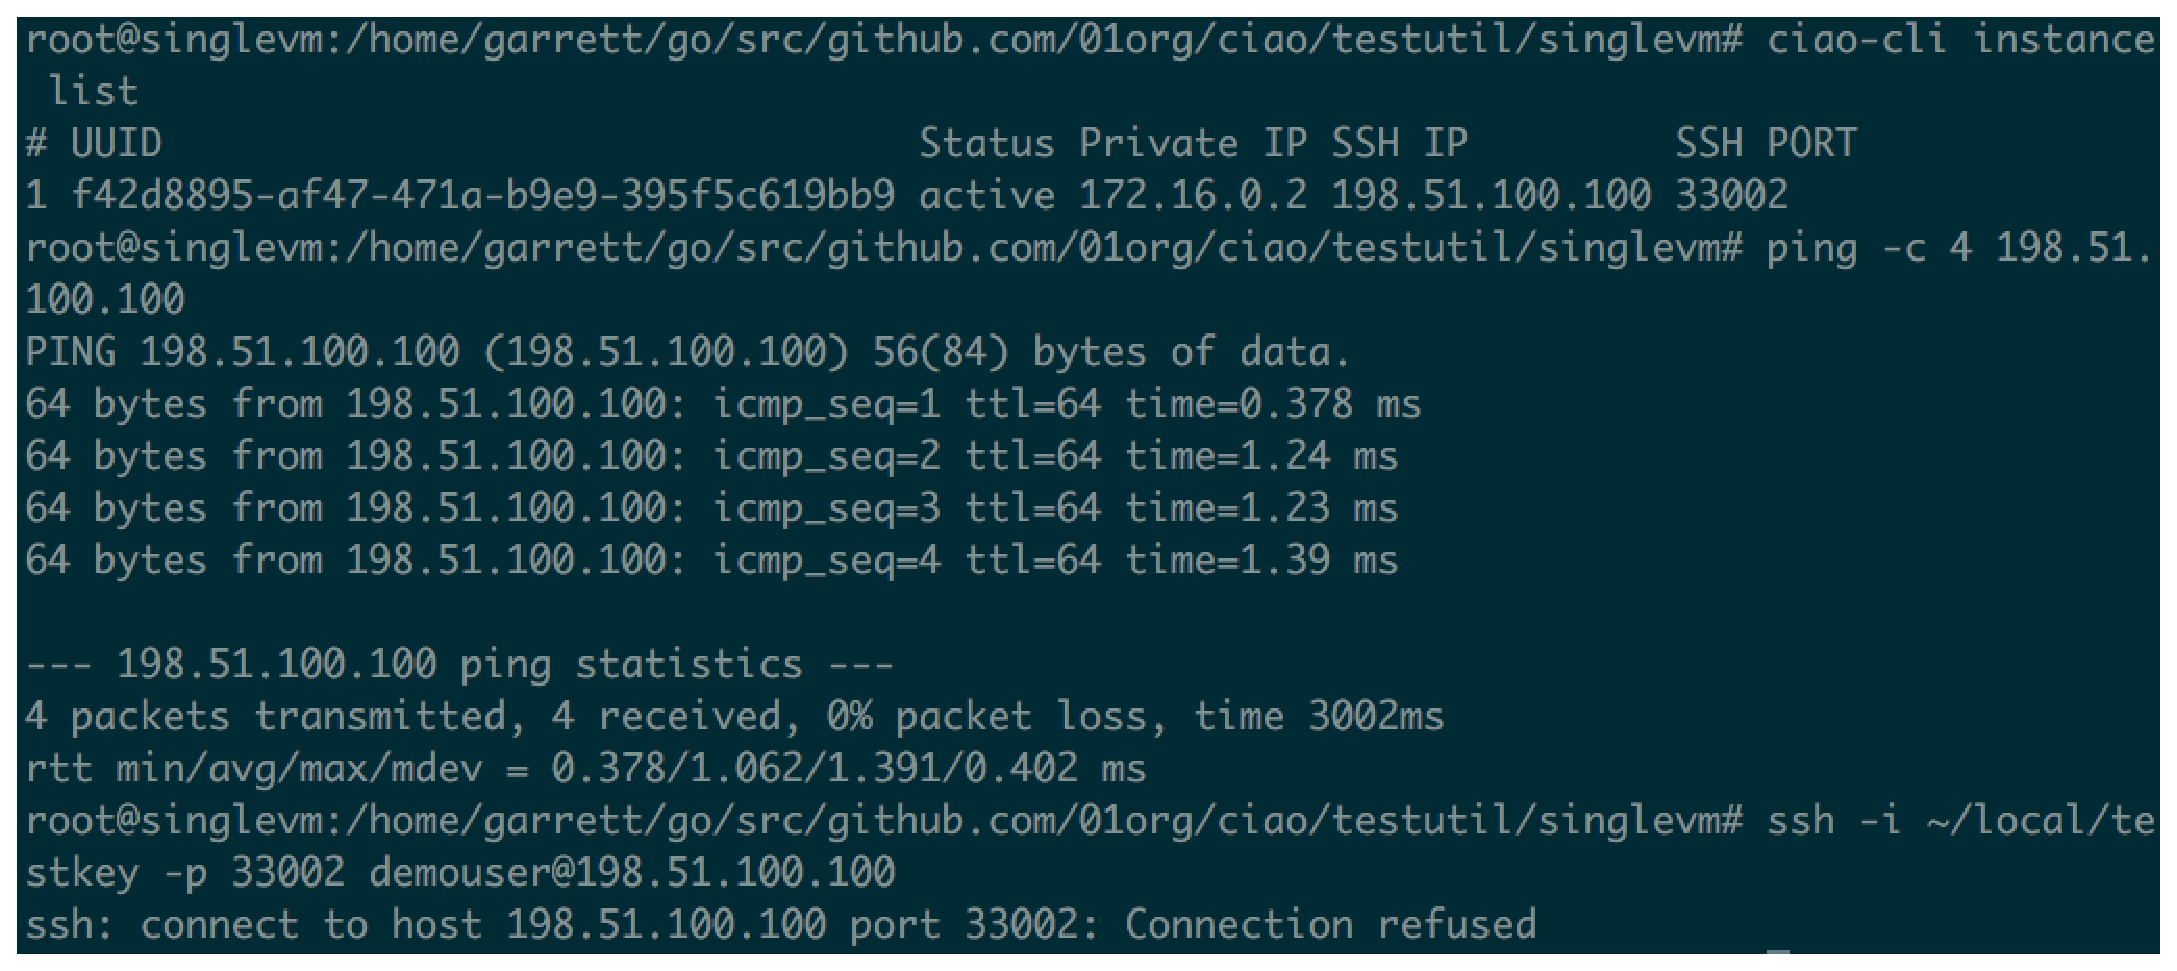
\includegraphics[scale=0.5]{./ssh-refused.eps}
\end{figure}

We continued to work on this problem until recently by trying to manipulate how
the controller nodes manage their virtual network interface cards (VNICs). Our
idea was that the VNICs could be made to communicate with the Open vSwitch
network objects if tracked correctly. This approach only broke our
implementation even more. We ended up rolling back our codebase to the point
where we could ping the instances but the ssh connection was refused.

\section{Issue}
After consulting with Manohar Castelino, a Principle Engineer at Intel and
original author of Ciao networking, he suspected that our project was very close
to working.  He suggested that we take a look at the maximum transmission unit,
or MTU, that Ciao was configured to use. MTU is the defined size of a packet or
IP frame that can be sent over the network~\cite{MTU}. This is configured on a
per-device basis. After standardizing MTU size within the ciao-down environment,
the results did not change. At present, our code is being reviewed by Manohar,
and we are working with him to figure out the problem.

%Code snippet of MTU setting

\section{Remaining Steps}

Our next steps are to work with Manohar to fix any further feedback he has for
us. As mentioned above, we are able to ping created instances, but not able to
ssh into them. As far as implementation goes, our sole remaining step is to fix
the ssh issue. The stretch goal of doing measurements on nvGRE and VxLAN are
untenable at this point in the term.

Beyond code, our next step is to present the project at the Engineering Expo on
May 19th.

\bibliographystyle{IEEEtran}
\bibliography{prog}

\end{document}
